\section{Tomasulo algorithm}

The Tomasulo Algorithm is a dynamic approach designed to enable execution to continue even in the presence of dependencies. 
It was developed at IBM, emerging three years after the CDC 6600, primarily for the IBM 360/91. 
Like its predecessors, its aim is to achieve high performance without the need for specialized compilers.

In Tomasulo's design, both the control logic and buffers are decentralized, contrasting with the centralized approach of a scoreboard. 
Buffers for operands are termed reservation stations, with each instruction represented as an entry within these stations.

\paragraph*{Register renaming}
In the Tomasulo Algorithm, operands are substituted with values or pointers, a technique known as Register Renaming. 
This approach helps in circumventing Write-After-Read and Write-After-Write hazards. 
Unlike traditional registers, reservation stations in Tomasulo are more versatile, enabling optimizations beyond the capabilities of a compiler.

Results are disseminated to other Functional Units via a Common Data Bus, which carries both data and its corresponding source. 
Additionally, Load/Store operations are treated as Functional Units within the algorithm.

\subsection{Tomasulo algorithm}
\begin{figure}[H]
    \centering
    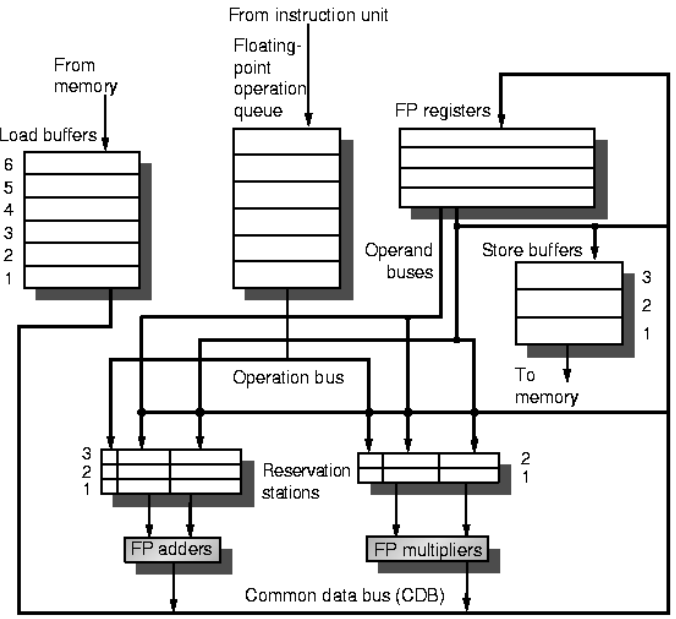
\includegraphics[width=0.5\linewidth]{images/tomasulo.png}
    \caption{Illustration of the Tomasulo Algorithm for a Floating Point Unit}
\end{figure}

\paragraph*{Reservation station}
A reservation station is equipped with the following components:
\begin{itemize}
    \item \textit{Tag}: identifies the reservation station.
    \item \textit{OP}: specifies the operation to be executed on the component.
    \item \textit{$V_j$, $V_k$}: values of the source operands.
    \item \textit{$Q_j$, $Q_k$}: pointers to reservation stations that produce $V_j$, $V_k$.
    \item \textit{Zero value}: indicates that the source operand is already available in either $V_j$ or $V_k$.
    \item \textit{Busy}: indicates whether the reservation station is currently occupied.
\end{itemize}
It's important to note that for each operand, only one of the V-field or Q-field is valid.


\paragraph*{Additional Components}
Aside from reservation stations, there are other essential elements within the Tomasulo Algorithm:
\begin{itemize}
    \item \textit{Register file and the store buffer}: both feature a Value (V) and a Pointer (Q) field. 
        The Pointer (Q) field corresponds to the number of the reservation station producing the result to be stored in the register file or store buffer. 
            If it's zero, it indicates no active instructions producing the result, implying that the register file or store buffer content is correct.
    \item \textit{Load buffers}: these buffers include an address field (A) and a busy field. 
        They are utilized for holding information related to memory address calculation for load/store operations. 
        Initially, they contain the instruction offset (immediate field). 
        After address calculation, they store the effective address.
    \item \textit{Store buffers}: similar to load buffers, store buffers also feature an address field (A).
        They are instrumental in managing store operations within the algorithm. 
\end{itemize}

\paragraph*{Algorithm}
The Tomasulo algorithm unfolds across three main stages:
\begin{itemize}
    \item \textit{Issue}: retrieve an instruction $I$ from the instruction queue. 
        If it's a floating-point operation, check if a reservation station is available (i.e., check for structural hazards). 
        Perform register renaming and resolve Write-After-Read hazards. 
        Handle Write-After-Write hazards by linking the register file to the instruction $I$ due to in-order issuance.
    \item \textit{Execution}: once both operands are available, execute the instruction. 
        If operands aren't ready, monitor the common data bus for results. 
        Delay execution until operands are ready to avoid Read-After-Write hazards. 
        Multiple instructions may become ready simultaneously for the same Functional Unit. 
        For load and store instructions, perform a two-step process: compute the effective address and store it in the load or store buffer. 
        Loads in the load buffer execute as soon as the memory unit is available, while stores in the store buffer wait until the value is ready to be stored before being sent to the memory unit.
    \item \textit{Write}: once the result is available, write it onto the common data bus. 
        From there, distribute it into the register file and all reservation stations (including store buffers) waiting for this result. 
        Stores write data to memory during this stage and mark reservation stations as available for the next instructions.
\end{itemize}

\paragraph*{Load and store}
Loads and stores undergo effective address computation in a functional unit before proceeding to their respective effective load and store buffers. 
Loads require a second execution step to access memory before transitioning to the Write Result stage to send the value from memory to the register file and/or reservation stations.

Stores complete their execution in their Write Result stage, which involves writing data to memory. 
All write operations occur in the Write Result stage, simplifying the Tomasulo algorithm.

Load and Store operations can be executed in a different order, provided they access different memory locations. 
Otherwise, hazards such as Write-After-Read or Read-After-Write may occur (with Write-After-Write if two stores are interchanged). 
Loads can be freely reordered.

To detect such hazards, the data memory addresses associated with any earlier memory operation must have been computed by the CPU. 

When a Load executes out of order with a previous Store, it's assumed that the address was computed in program order. 
Once the Load address is computed, it's compared with the address fields in active store buffers. 
If there's a match, the Load isn't sent to the Load buffer until the conflicting store completes.

Stores must check for matching addresses in both load and store buffers (dynamic disambiguation), an alternative to the static disambiguation performed by the compiler. 
However, this approach requires a significant amount of hardware. 
Each reservation station must contain a fast associative buffer, and a single common data bus may limit performance.

\subsection{Tomasulo and scoreboard comparison}
The key features of Tomasulo algorithm are: 
\begin{itemize}
    \item Issue window size of 14.
    \item No issue on structural hazards.
    \item Write-After-Read and Write-After-Write hazards are avoided with renaming.
    \item Results are broadcasted from functional units.
    \item Control is distributed across reservation stations.
    \item Allows loop unrolling in hardware.
\end{itemize}
The key features of scoreboard algorithm are: 
\begin{itemize}
    \item Issue window size of 5.
    \item No issue on structural hazards.
    \item Stall the completion for WAW and WAR hazards.
    \item Results are written back on registers.
    \item Control is centralized through the Scoreboard.
\end{itemize}
Both approaches distribute control and buffers with functional units versus centralizing them in the scoreboard. 
Reservation stations in Tomasulo serve as buffers for pending operands. 
Registers in instructions are replaced by values or pointers to reservation stations, a technique known as register renaming, which helps avoid WAR and WAW hazards. 
Tomasulo can utilize more reservation stations than registers, enabling optimizations beyond compilers' capabilities.

Results are sent to functional units from reservation stations, not through registers, via a Common Data Bus that broadcasts results to all functional units. 
Additionally, both load and stores are treated as functional units with associated Reservation Stations.

Furthermore, in Tomasulo, integer instructions can proceed past branches, allowing floating-point operations beyond the basic block in the floating-point queue.